\chapter{FoodOn}

\section{Ontologia}
\index{Ontologia}

La necessit� di rappresentare la conoscenza del cibo � fondamentale per molte attivit� umane tra cui agricoltura, medicina, ispezione della sicurezza alimentare, modelli di acquisto e sviluppo sostenibile.
FoodOn � una risorsa ontologica completa e open-source composta da sfaccettature gerarchiche di termini che comprendono ingredienti di base delle materie prime alimentari, termini di processo per l'imballaggio, la cottura e la conservazione e una variet� di schemi dei tipi di prodotto di livello superiore in base ai quali i prodotti alimentari possono essere classificati.
\begin{figure}[!h]
    {\begin{center}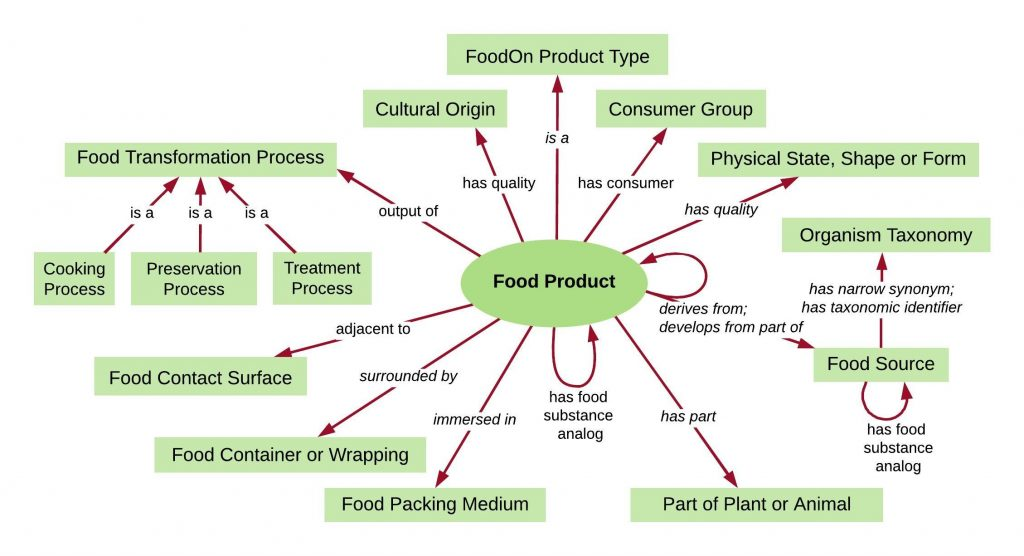
\includegraphics[width=14cm]{FIGURE/figure-1-foodon-food-schema-2-1024x556.jpeg}\end{center}}
\caption{\textbf{Diagramma di ``Food Product"} - Lo schema dei prodotti alimentari di FoodOn deriva principalemnte dalle sfaccettature della descrizione degli alimenti di LanguaL con l'aggiunta di relazioni ontologiche tra un prodotto alimentare e le relative qualit� descrittive, componenti e processi. \label{tab1}}
\end{figure}
Ad ora FoodOn � fornito sotto forma di Web Ontology Language (OWL) tramite repository GitHub del progetto stesso: \href{https://github.com/FoodOntology/foodon}{\textit{\underline{github.com/FoodOntology/foodon}}}\\


L'ultima versione pu� anche essere esplorata tramite servizi di ricerca ontologica come:
\begin{itemize}
\item BioPortal, \href{https://bioportal.bioontology.org}{\textit{\underline{bioportal.bioontology.org}}}
\item European Bioinformatics Institute Ontology Lookup Service (EMBL-EBI), \href{https://www.ebi.ac.uk/ols/}{\textit{\underline{www.ebi.ac.uk/ols/}}}
\item Ontobee, \href{http://ontobee.org}{\textit{\underline{ontobee.org}}}
\item AgroPortal, \href{http://agroportal.lirmm.fr/}{\textit{\underline{agroportal.lirmm.fr}}}
\end{itemize}
  
\subsection{FoodOn e LanguaL}
\index{FoodOn e LanguaL}

\section{Struttura}
\index{Struttura}
\section{Funzionalit�}
\index{Funzionalit�}

